\newpage

\section{Description détaillée du nouveau logiciel}
\paragraph{}
Dans cette partie, nous allons explorer la mécanique interne du programme VisualImpro, tout d'abord de façon générale, puis nous allons entrer en détail dans les composantes principales de ce programme, afin que l'on puisse avoir une vision d'ensemble claire et précise des fonctionnalités. 
\subsection{Le point d'entrée du programme}
\paragraph{}
Lorsque le programme est lancé via l'éxécutable, il se passe alors plusieurs choses :
\begin{itemize}
    \item Les paramètres sont chargés sur BELA à travers un fichier de configuration. Ce fichier contient les différentes entrées (audio, analogiques ou fichiers \verb!.wav!) que Bela va traiter ainsi que les différents traitements qui seront appliqués à ces entrées. 
    \item Si des fichiers \verb!.wav! sont indiqués dans le fichier de configuration, alors ceux-ci seront aussi chargés sur BELA.
\end{itemize}
\paragraph{}
Ensuite, le programme VisualImpro de BELA débute. La première tâche effectuée par la fonction \verb!main! est de récupérer le fichier de configuration et de stocker les divers paramètres écrits à l'intérieur de celui-ci. Puis à l'aide des différents paramètres, la deuxième tâche de la fonction \verb!main!
va être d'initialiser les éléments correspondants. Enfin, la dernière tâche de la fonction \verb!main! va être de donner la main à la fonction principale de traitement audio à travers l'appel \verb!Bela_startAudio!. Avec cet appel, on passe à la fonction principale qui se situe dans le fichier \verb!render.cpp! et qui porte le nom de \verb!render!.
\subsection{La boucle de traitement principale}
\paragraph{}
Avant de passer directement à la fonction \verb!render!, le programme va passer par la fonction \verb!setup! qui va initialiser toutes les structures nécessaires au bon déroulement de la fonction \verb!render!, ainsi qu'un autre élément central du programme, les tâches auxiliaires. Ces tâches auxiliaires, qui font partie des éléments fournis par le framework Bela, permettent au programmeur de créer des segments de code qui seront exécutés en parallèle, ce qui permet d'alléger le travail effectué dans la fonction \verb!render!, et donc d'éviter de créer des latences qui pourraient perturber le retour en temps réel. C'est pour cela que l'on initialise des tâches auxiliaires dans la fonction \verb!setup! en spécifiant le code qui sera éxécuté dans chacune d'entre elles. Parmi les 3 différentes tâches présentes dans le code, seules 2 sont intéressantes : la tâche qui aura pour but de remplir les tampons, et celle qui traitera un tampon rempli. La troisième consiste à appliquer des effets sur un tampon, mais ce n'est pas un aspect du projet qui sera traité.
\paragraph{}
Par la suite, la fonction principale \verb!render! va être appelée en chaîne, jusqu'à ce qu'un signal lui indique qu'elle peut s'arrêter. Dans cette fonction, il va se passer plusieurs choses : 
\begin{itemize}
    \item Si les différents tampons ne sont pas tous remplis, alors on déclenche la tâche auxiliaire de remplissage,
    \item Une fois que les tampons sont remplis, on déclenche la tâche auxiliaire de traitement,
    \item Enfin, on récupère les signaux après traitement et on les envoie sur la sortie audio de Bela.
\end{itemize}
\begin{figure}[H]
    \centering
    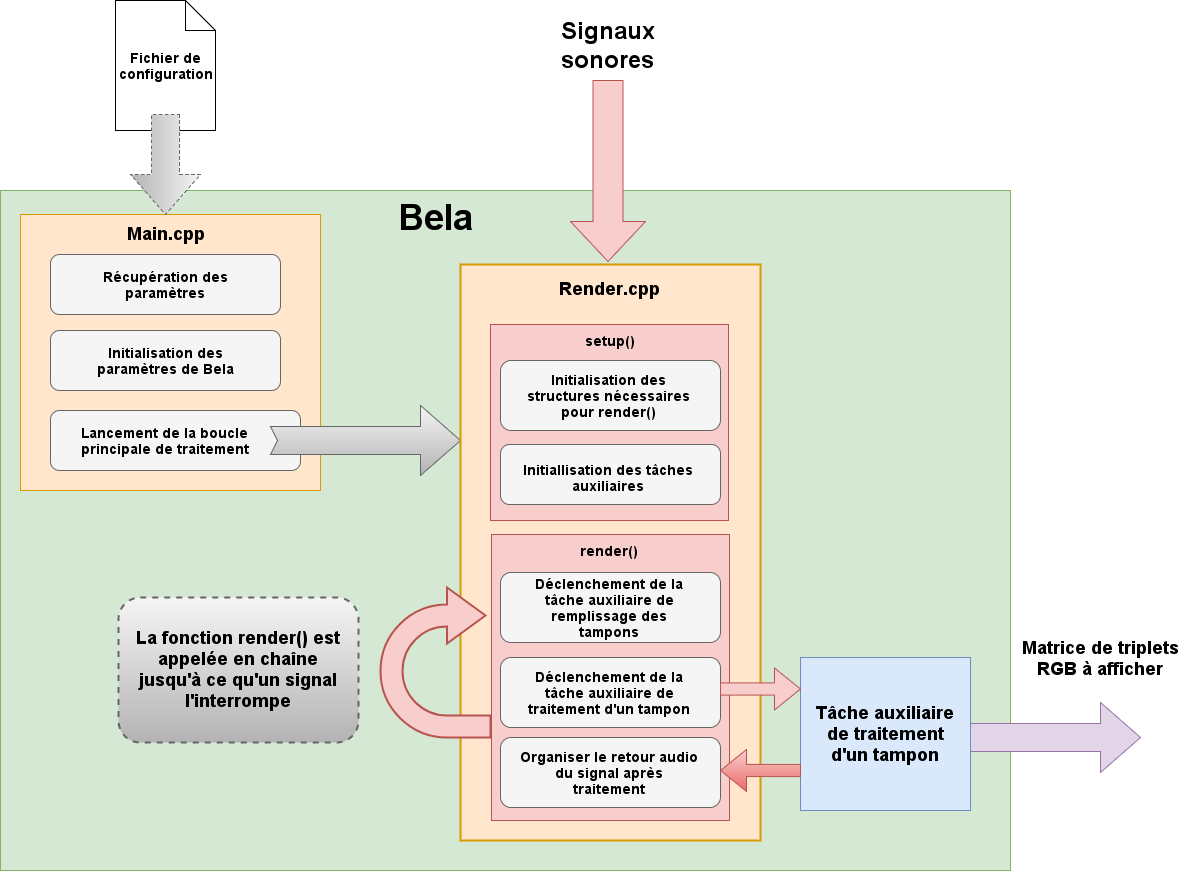
\includegraphics[scale=0.4]{assets/render.png}
    \caption{Fonctionnement des fonctions principales de l'outil}
    \label{focntionnement main render}
\end{figure}
\subsection{La tâche auxiliaire de traitement}
\paragraph{}
Dans ce mémoire, on ne traitera que la tâche auxiliaire concernant le traitement, car la tâche auxiliaire de remplissage de tampon est réalisée par le code de la classe \verb!SampleStream! qui est une classe qui est fournie sur le site de Bela \cite{BELA}. Son contenu n'est pas voué à être modifié, mais il reste tout de même essentiel à la mécanique générale du programme.
\paragraph{}
La tâche auxiliaire de traitement du contenu audio est liée à une classe importante de notre outil, la classe \verb!ProcessMultiCorrel!. C'est cette classe qui va prendre un fragment des entrées, stocké dans un tampon, et qui va appliquer différents traitements sur ce tampon. Le traitement va se dérouler en 4 étapes exécutées séquentiellement.
\subsubsection{Le pré-traitement}
\paragraph{}
La fonction de pré-traitement va servir à dégager une caractéristique du signal. Parmi les fonctions de pré-traitement dsiponibles, il y a la récupération de l'énergie du signal et le calcul de l'enveloppe du signal. Le graphique suivant représente l'enveloppe supérieure (en rouge) et l'enveloppe inférieure (en jaune) d'un signal (en bleu). \cite{ENV}
\begin{figure}[H]
    \centering
    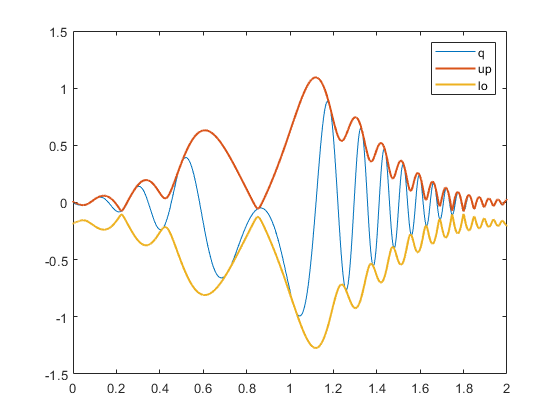
\includegraphics[scale=0.6]{assets/signal-enveloppe.png}
    \caption{Représentation de l'enveloppe d'un signal}
    \label{enveloppe signal}
\end{figure}
\paragraph{}
Le bénéfice du calcul de l'enveloppe est d'avoir des valeurs plus stables, ce qui évite d'avoir en sortie des résultats extrêmement chaotiques.
\paragraph{}
En ce qui concerne l'énergie du signal, le principe est le suivant : on va découper le tampon en blocs, et pour chaque bloc, on va calculer la moyenne des valeurs du tampon assoicées au bloc au carré. Cela a pour but d'éliminer les valeurs négatives du signal et de réduire la taille de l'échantillon à traiter,
ce qui va réduire les temps de calcul, donc les latences.
\subsubsection{Le calcul du coeffcient de corrélation}
\paragraph{}
C'est à cette étape que l'on va calculer le coefficient de corrélation. Les coefficients sont calculés pour chaque paire d'entrées, donc pour N entrées nous obtenons une matrice de coefficients $N \times N$ symétrique où la diagonale n'est significative. Comme indiqué dans l'introduction de ce mémoire, la vision que l'on a d'une bonne improvisation est totalement subjective. De ce fait, les fonctions calculant un coefficient de corrélation n'ont pas l'obligation d'être rigoureuses (physiquement et mathématiquement parlant). Pour illustrer notre propos, nous avons mis à disposition une fonction retournant des valeurs aléatoires (toujours comprises entre 0 et 1 dans un soucis de généricité), ce qui donnera un retour visuel et audio tout aussi aléatoire.
\subsubsection{La modification du volume}
\paragraph{}
Après avoir obtenu un coefficient de corrélation (et quelque soit la manière), on va modifier les volumes des entrées en fonction des coefficients obtenus. À ce jour, il y a deux fonctions de mixage des volumes disponibles : une qui va augmenter le volume proportionnellement par rapport au  coeffcient de corrélation, et sa fonction de mixage complémentaire (qui va diminuer le volume d'une entrée proportionnellement à son coeffcient de corrélation). Pour chaque entrée, le résultat obtenu est la moyenne de ses coefficients de corrélation obtenus avec toutes les autres entrées.
\subsubsection{La traduction en triplet RGB}
\paragraph{}
Pour obtenir un retour graphique pertinent, la matrice de coefficients de corrélation va être associée à une couleur dans une échelle indiquée en paramètre. Les échelles de couleur disponibles à ce jour sont l'échelle noire/blanche et l'échelle rouge/vert. Les coefficients vont alors être traduits en triplets RGB, afin qu'ils puissent être affichés simplement par la suite.
%Screenshots matrice avec les deux échelles de couleur
\paragraph{}
Enfin, après avoir réalisé ces 4 étapes, l'ultime travail de la tâche auxiliaire est d'envoyer la matrice de triplets RGB via une connexion TCP vers l'entité s'occupant de l'affichage (serveur NodeJS ou application QT).
\begin{figure}[H]
    \centering
    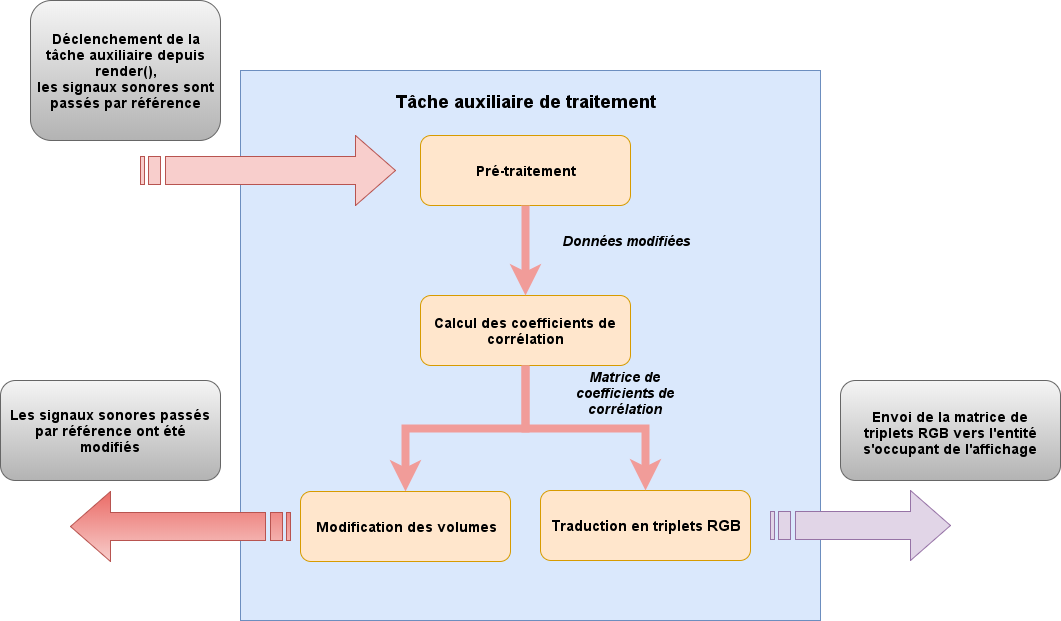
\includegraphics[scale=0.45]{assets/auxtask.png}
    \caption{Déroulement de la tâche auxiliaire de traitement}
    \label{aux task}
\end{figure}

